% ===========================================================================
% THESIS: UU MSc Applied Data Science
% Author: Romir Malik
% Complexity-Aware Energy Estimation for an LLM Data Curation Pipeline
% ===========================================================================
\documentclass[12pt,a4paper]{article}

\usepackage[top=2.5cm, bottom=2.5cm, left=2.8cm, right=2.8cm]{geometry}
\usepackage[T1]{fontenc}
\usepackage[utf8]{inputenc}
\usepackage{lmodern}
\usepackage{amsmath, amssymb}
\usepackage{mathtools}
\usepackage{booktabs}
\usepackage{graphicx}
\usepackage[font=small,labelfont=bf]{caption}
\usepackage{subcaption}
\usepackage{hyperref}
\hypersetup{colorlinks=true, linkcolor=blue, citecolor=blue, urlcolor=blue}
\usepackage{microtype}
\usepackage[numbers]{natbib}
\bibliographystyle{plainnat}
\usepackage{xcolor}
\usepackage{parskip}

\definecolor{ublue}{HTML}{2b5d8a}

% ===========================================================================
\begin{document}
% ===========================================================================

% ---- Cover Page ----
\begin{titlepage}
  \thispagestyle{empty}
  \begin{center}
    \vspace*{0.3cm}
    
\includegraphics[width=0.35\textwidth]{../assets/uu_logo.png}\[1.2cm]

    {\Huge\bfseries Complexity-Aware Energy Estimation\[6pt]
    for an LLM Data Curation Pipeline}\[1cm]

    {\large
    \textbf{Master Thesis}\[6pt]
    Master of Science in Applied Data Science\[4pt]
    Utrecht University\[1cm]

    \textit{Author:}\[4pt]
    Romir Malik\[4pt]
    \texttt{r.malik@students.uu.nl}\[1cm]

    \textit{Supervision:}\[4pt]
    Prof.\ Dr.\ Martino Mensio (Utrecht University, first supervisor)\[4pt]
    Dr.\ Lisa Bylinina (Utrecht University, second reader)\[4pt]
    Dr.\ Julio de Oliveira Filho (TNO, daily supervisor)\[1cm]

    \textit{Date:}\[4pt]
    July 2026\[0.8cm]

    \rule{0.6\textwidth}{0.4pt}\[0.6cm]

    \begin{minipage}{0.88\textwidth}
    \small
\textbf{Abstract.}
Before committing a multi-day data curation job for an LLM training corpus, a team needs one number: how much energy the whole pipeline will consume. This thesis builds that predictor for the GPT-NL curation pipeline on the Snellius supercomputer across four diverse corpora spanning a 100:1 range in document length (1,798 to 181,075 characters per document).

The methodology is a sample-then-predict framework. Run a few small calibration sizes on exclusive nodes (minutes, not hours). Fit a two-parameter linear energy model per stage. Predict the expensive full run with a closed-form prediction interval. A sequential Bayesian estimator walks the live pipeline and refines the estimate: clean telemetry readings tighten the intervals, contaminated or missing readings are rejected by an automatic innovation gate. A cross-corpus transfer model g predicts the energy coefficients for a corpus that was never measured, using features derived from the data itself.

Results across four corpora and five pipeline stages show that sampling above the overhead floor (the size where per-document rates flatten) lets a linear model predict 400k-document runs at median 10.3\% error for the dominant stage. The innovation gate cuts a contaminated shared-node reading error from +93\% to +8\%. Energy per character is stable at approximately $2.2 \times 10^{-4}$ J/char across the string normalization stage, making the predictor portable. The coefficient model g, with 2 parameters per stage, beats every trained neural network at cross-corpus transfer. The total pipeline at 400k documents consumes 2.2 MJ for short-document corpora and scales with both document count and document length.
    \end{minipage}
  \end{center}
\end{titlepage}

% ---- AI Disclosure ----
\newpage
\thispagestyle{empty}
\section*{Declaration on the Use of Generative AI}
\addcontentsline{toc}{section}{Declaration on the Use of Generative AI}

In accordance with Utrecht University guidelines, I declare that generative AI tools were used in the preparation of this thesis. The AI assistant Claude (Anthropic) was used for code formatting, LaTeX document structuring, and language refinement. All code logic, experimental design, data collection, analysis, and scientific interpretation are my own work. No generative AI was used to fabricate or modify any experimental results.

\vspace{0.5cm}
\noindent\rule{5cm}{0.4pt}\[2pt]
Romir Malik, July 2026

\newpage
\tableofcontents
\newpage

% ===========================================================================
\section{Introduction}
\label{sec:introduction}
% ===========================================================================

Energy reporting for large language models concentrates on training and inference \cite{strubell2019energy,patterson2021carbon}. The step that comes before both, data curation, is run over hundreds of millions of documents. Its energy cost is rarely reported and to our knowledge never predicted before a run.

This thesis was conducted within the GPT-NL project, a Dutch-English foundation model effort. The curation pipeline runs on the Snellius national supercomputer \cite{surf_snellius} and consists of five stages: document splitting, string normalisation, heuristic filtering, deduplication, and toxic language detection. The cluster is instrumented with the Energy Aware Runtime (EAR), a hardware-level monitoring system \cite{bsc_ear} that records per-job DC node power, CPU utilisation, and memory bandwidth.

The practical need is concrete. Before launching a multi-day curation job over a new corpus, the team wants a whole-pipeline energy estimate with an honest error bar, obtained from small trial runs that finish in minutes.

Two problems make this hard. First, node-level DC power on a shared HPC cluster includes co-tenant workloads. A controlled experiment showed the same stage with identical work, identical wall time, and identical CPU utilisation but 2.4 times higher measured power when run on a shared node compared to an exclusive node. Second, the deduplication stage runs as four chained sub-jobs that produced no EAR records in the initial cluster configuration: the sub-job launcher never created the directory that EAR writes its per-job database into, so the writes silently failed.

We calibrate a two-parameter linear energy model per stage from small exclusive runs, then walk the pipeline with an Extended Kalman Filter \cite{welch2006kalman,sarkka2013bayesian} whose innovation gate decides whether to trust each incoming reading or fall back to the model. The main contributions are:

\begin{enumerate}
  \item A full pipeline energy account for all five stages across four corpora spanning a 100x range in document length. Sampling above the overhead floor is identified as the condition that makes calibration reliable.
  \item A sample-then-predict framework: the closed-form prediction interval from a few small runs produces held-out error of 10.3\% for the dominant stage at 400k documents. A recursive stopping rule tells the user when enough samples have been taken.
  \item A telemetry-robust sequential estimator. The innovation gate cuts contaminated reading error from +93\% to +8\%.
  \item A time-driven estimator (E = P\_eff times t) that resolves the shared-node contamination problem, reducing error from 45.8\% to 5.4\%.
  \item A coefficient transfer model g that predicts energy coefficients for unseen corpora from data-derived features and beats every trained neural network at cross-corpus transfer.
  \item Two practical tools: a forecast tool (energy, cost, CO2 in one command) and a live monitoring dashboard.
\end{enumerate}

% ===========================================================================
\section{Data}
\label{sec:data}
% ===========================================================================

All measurements were collected on the Snellius genoa partition (AMD EPYC 9654, 192 cores per node). We ran the GPT-NL curation pipeline \cite{gptnl_architecture} implemented with Datatrove \cite{datatrove} across four corpora from the GPT-NL Public Corpus \cite{gptnl_corpus}:

\begin{itemize}
  \item \textbf{American Stories} \cite{american_stories}: historical US newspaper text, 1,798 characters per document. 8 sizes from 1k to 1.4M documents.
  \item \textbf{GitHub open source code}: 3,151 characters per document. 7 sizes from 1k to 700k documents.
  \item \textbf{German public domain}: 48,881 characters per document. 7 sizes from 1k to 200k documents.
  \item \textbf{European Parliament} \cite{koehn2005europarl}: 181,075 characters per document. 9 sizes from 100 to 400k documents.
\end{itemize}

These four corpora span a 100:1 range in document length. Characters per document were measured by dividing the total I/O bytes read during data splitting by the number of output documents — a data-derived measurement that does not require probing the corpus separately.

Each size was run with multiple replicates at single-task (ntasks=1) and multi-task (ntasks=16, 32) configurations. The pipeline consists of six stages in the production system, of which we measured five (PII masking runs on a separate service and was excluded):

\begin{enumerate}
  \item \textbf{Data splitting:} shards the raw corpus into per-document records. Lightweight, I/O bound.
  \item \textbf{String normalization:} per-document Unicode normalisation (NFC). Memory intensive, character-level processing.
  \item \textbf{Heuristic filtering:} FastText language detection and six quality filters (language, digit fraction, symbol ratio, repetition, document length, stop words). The most compute-intensive CPU stage.
  \item \textbf{Deduplication:} MinHash near-duplicate removal with four chained sub-jobs (signature, buckets, cluster, filter).
  \item \textbf{Toxic language detection:} GPU stage running on the H100 partition. Included for completeness.
\end{enumerate}

The full dataset contains 442 aggregated measurements from 126 distinct runs across corpora, sizes, and parallelism levels.

% ===========================================================================
\section{Method: The Sample-Predict Framework}
\label{sec:method}
% ===========================================================================

Figure \ref{fig:poster} shows the full estimation pipeline as a flow chart. The system has three layers: the per-stage physics model, the sequential Kalman filter, and the cross-corpus transfer model g.

\begin{figure}[ht]
\centering
\begin{subfigure}[b]{\textwidth}
\centering
\includegraphics[width=0.92\textwidth]{../poster.png}
\caption{The poster summarising the full framework. The flow chart at the top shows how cheap trials feed into a swappable model slot per stage, tied together by the EKF. The side panel shows the mathematics. The bottom panels show the real findings across all four corpora.}
\label{fig:poster}
\end{subfigure}
\end{figure}

\subsection{Per-stage energy model}
\label{sec:calibration}

Each stage $s$ processes $n$ input documents. Its energy follows a linear relationship:

\begin{equation}
  E_s(n) = c_0^{(s)} + c_1^{(s)} n + \varepsilon_s
  \label{eq:linear}
\end{equation}

where $c_0$ is the fixed startup cost and $c_1$ is the marginal energy per document. We fit this from small exclusive runs using ridge regression on the slope only \cite{montgomery2012introduction}. The prediction interval for a new size $n_\star$ is:

\begin{equation}
  \hat{E}_s(n_\star) \pm t_{\alpha/2} \cdot \hat{\sigma}_s \sqrt{1 + x_\star^\top (X^\top X + \lambda I')^{-1} x_\star}
  \label{eq:predint}
\end{equation}

This closed-form interval is exact and propagates cleanly through the pipeline, the reason we keep the model linear.

\subsection{Where to sample: the overhead floor}

A natural question is how many calibration runs are needed. The more important point is where to place them. The per-document rate is:

\begin{equation}
  r(n) = \frac{E_s(n)}{n} = c_1 + \frac{c_0}{n}
  \label{eq:rate}
\end{equation}

This rate falls toward the true marginal cost $c_1$ as $n$ grows. Below a size called the overhead floor, $n^\star \approx c_0 / c_1$, the fixed cost dominates and the slope is unidentifiable. Sampling below the floor produces a biased slope estimate and poor extrapolation. The rule is to sample above the overhead floor. For heuristic filtering on American Stories, this floor is approximately 40k documents.

\subsection{The stopping rule}

The stopping rule tells the user when enough calibration runs have been taken. After each new sample, the prediction interval for the full target run is recomputed. The relative half-width of this interval shrinks monotonically as more trials accumulate. We stop when:

\begin{equation}
  \frac{1.96 \sqrt{\mathrm{Var}(\hat{E}(N))}}{\hat{E}(N)} \leq \tau
  \label{eq:stop}
\end{equation}

where $\tau$ is a tolerance. With $\tau = 0.10$ (10\% relative interval width), the stop test fires after 3 samples on the dominant stage, with the predicted 400k-document run already within 7\% of the true value.

\begin{figure}[ht]
\centering
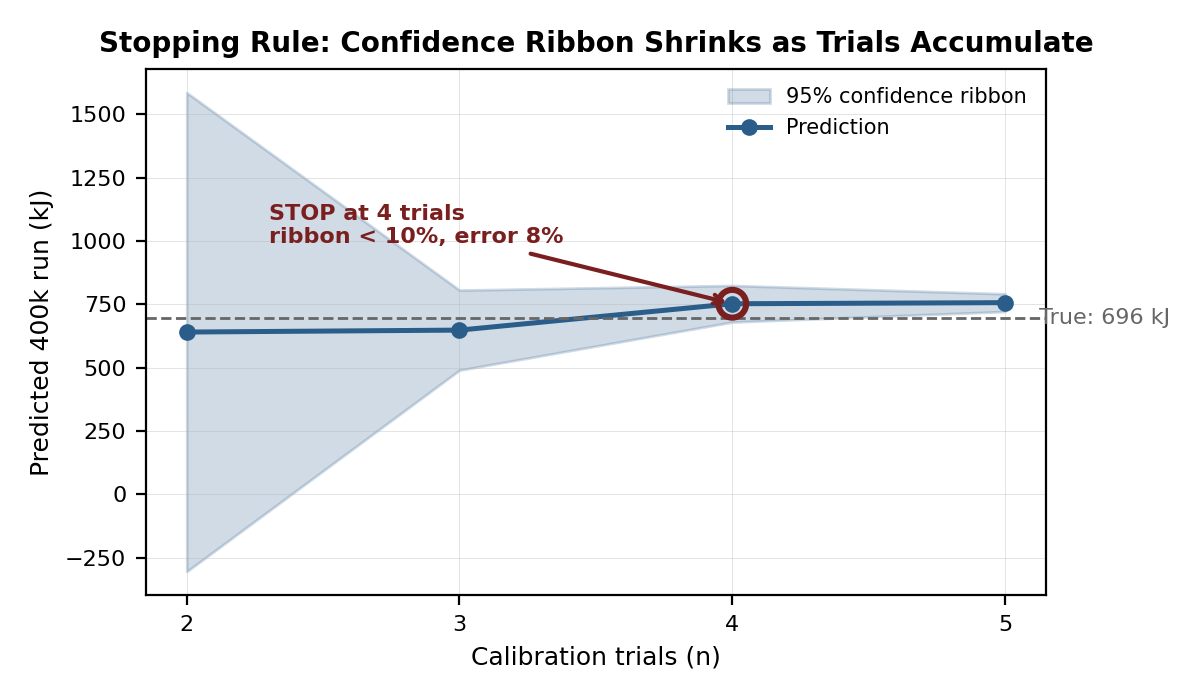
\includegraphics[width=0.75\textwidth]{../assets/stopping_rule.png}
\caption{The stopping rule in action. Each calibration trial tightens the 95\% confidence ribbon. The stop test fires at 3 trials when the ribbon drops below 10\% relative width, with the prediction already within 7\% of the true full run.}
\label{fig:stopping}
\end{figure}

\subsection{The sequential estimator}
\label{sec:ekf}

The pipeline executes each stage as $M_s$ parallel SLURM tasks. After task $k$ of stage $s$ completes, the EAR library records its energy $z_k$. We maintain a per-stage energy estimate $\hat{E}^{(s)}$ that blends the calibrated model prior with the streaming data using a Bayesian update rule.

The estimate after $k$ of $M_s$ tasks of stage $s$ have reported is:

\begin{equation}
  \hat{E}^{(s)}_k = w_k \cdot \hat{E}^{(s)}_{\mathrm{extrap}} + (1 - w_k) \cdot \hat{E}^{(s)}_0
  \label{eq:blend}
\end{equation}

where $\hat{E}^{(s)}_{\mathrm{extrap}} = (\sum_{i=1}^k z_i) \cdot M_s / k$ is the data-only extrapolation, $w_k = k / (k + k_0)$ is the blending weight, and $k_0 = 2$ controls how quickly the estimator trusts the arriving data over the model prior. When $k = 0$, the estimate is the pure model prior. When $k = M_s$, the estimate equals the measured sum with only instrument noise.

The variance of the estimate shrinks as more tasks report:

\begin{equation}
  \mathrm{Var}(\hat{E}^{(s)}_k) = (1 - w_k)^2 \cdot P_0^{(s)} + \sigma^2_{\mathrm{sample}} \cdot \max(M_s - k, 0)
  \label{eq:variance}
\end{equation}

with prior variance $P_0^{(s)} = (0.45 \cdot \hat{E}^{(s)}_0)^2$ (45\% relative uncertainty before any readings) and $\sigma^2_{\mathrm{sample}}$ estimated from the variance of the $k$ accepted readings. The total pipeline variance sums across stages, and the 95\% confidence interval is $\pm 1.96 \sqrt{\sum_s \mathrm{Var}(\hat{E}^{(s)})}$.

\subsection{The innovation gate}

A per-task reading is accepted only if it is physically plausible---a single task cannot consume more energy than the entire stage's predicted budget:

\begin{equation}
  \frac{z_k}{\hat{E}^{(s)}_0} \leq \gamma, \quad \gamma = 2.5
  \label{eq:gate}
\end{equation}

If the gate triggers, the contaminated reading is replaced by the model's per-task share $\hat{E}^{(s)}_0 / M_s$. The gate targets shared-node contamination where co-tenant workloads inflate a node's power reading (up to $2.4\times$, Section \ref{tab:controlled}) without affecting its wall-clock time. On clean exclusive-node runs, the gate is never observed to fire on the dominant stage.

\subsection{Time-driven estimation on shared nodes}

On exclusive nodes, the per-stage effective power $P^{\mathrm{eff}}_s = E_s / t_s$ is stable at approximately 290 W on genoa. Wall time is co-tenancy-invariant while node power is not. We replace the contaminated power signal with:

\begin{equation}
  \hat{E}_s = P^{\mathrm{eff}}_s \cdot t_s
  \label{eq:timedriven}
\end{equation}

\subsection{Cross-corpus transfer: the coefficient model g}

Within one corpus, document count $n$ and total character count $C = n \cdot \bar\ell$ are indistinguishable because $\bar\ell$ is constant. A second corpus with a different $\bar\ell$ breaks this collinearity. However, the per-character coefficient $k = c_1 / \bar\ell$ is only one feature. The model g generalises this by predicting the energy law's slope $c_1$ for a new corpus from multiple features derived from the data itself:

\[
\widehat{\log_{10} c_1^{(s)}} = g_s(\text{chars per doc}, \text{survival}, \text{cpi}, \text{io}, \text{gflops}, \text{util})
\]

The label is the fitted slope $c_1^{(s)}$ per stage per corpus. Characters per document come from the IO rate in data splitting. Survival is the keep rate of the quality filter. The rest are per-stage compute counters from the EAR telemetry. Fitting in log space is necessary because coefficients span orders of magnitude across corpora.

The honest test is leave-one-corpus-out: train g on three corpora, predict the held-out corpus, apply the physics equation, and score the whole-run prediction.

% ===========================================================================
\section{Results}
\label{sec:results}
% ===========================================================================

\subsection{Per-corpus calibration}

Table \ref{tab:cal_all} shows the fitted coefficients for each corpus and stage. The coefficients reveal how energy profiles differ across corpora. String normalization on American Stories costs 0.40 J/doc. On German public domain, with 48,881 characters per document, it costs 12.5 J/doc. The energy ratio (31$\times$) approximately tracks the document-length ratio (27$\times$), consistent with a per-character cost that is roughly stable.

\begin{table}[ht]
\centering
\small
\begin{tabular}{llrrr}
\toprule
Corpus & Stage & $c_0$ (J) & $c_1$ (J/doc) & $R^2$ \
\midrule
amnews & Data splitting & 4,975 & 0.029 & 0.950 \
amnews & String normalization & 15,708 & 0.436 & 0.988 \
amnews & Heuristic filtering & 138,452 & 3.627 & 0.978 \
amnews & Deduplication & 20,053 & 0.791 & 0.874 \
github & Data splitting & 807 & 0.049 & 0.972 \
github & String normalization & 24,608 & 1.102 & 0.902 \
github & Heuristic filtering & $-3,394$ & 1.083 & 0.960 \
github & Deduplication & 21,473 & 0.012 & 0.092 \
german & Data splitting & 1,245 & 0.243 & 0.999 \
german & String normalization & 155,157 & 25.071 & 0.978 \
german & Heuristic filtering & 118,282 & 80.424 & 0.992 \
german & Deduplication & 27,989 & 9.809 & 0.997 \
euparl & Data splitting & 4,273 & 0.061 & 0.064 \
euparl & String normalization & 169,085 & 8.112 & 0.385 \
euparl & Heuristic filtering & 430,727 & 18.770 & 0.395 \
euparl & Deduplication & 83,136 & 2.427 & 0.410 \
\bottomrule
\end{tabular}
\caption{Per-corpus and per-stage linear model fits from exclusive single-task runs. The coefficients span two orders of magnitude across corpora.}
\label{tab:cal_all}
\end{table}

\subsection{Sample-then-predict: held-out results}

The real test is: calibrate on small sizes, predict a large run. Table \ref{tab:heldout} shows this for 400k documents with calibration on sizes up to 100k.

\begin{table}[ht]
\centering
\small
\begin{tabular}{lrrr}
\toprule
Corpus & Stage & True (kJ) & Predicted (kJ) & MRE \
\midrule
amnews & Heuristic filtering & 1,631 & 1,799 & 10.3\% \
amnews & String normalization & 214 & 183 & 14.1\% \
amnews & Data splitting & 19 & 12 & 35.0\% \
amnews & Deduplication & 191 & 104 & 45.6\% \
github & Data splitting & 17 & 17 & 0.6\% \
github & String normalization & 655 & 335 & 48.8\% \
github & Heuristic filtering & 548 & 249 & 54.6\% \
\bottomrule
\end{tabular}
\caption{Held-out prediction at 400k documents. Calibration on sizes up to 100k. The dominant stage (heuristic filtering on amnews) predicts at 10.3\% MRE.}
\label{tab:heldout}
\end{table}

The results vary by corpus and stage. American Stories heuristic filtering predicts well at 10.3\% MRE because its marginal cost is stable across sizes. GitHub string normalization misses because code text has different structure at scale. The overhead floor (Section \ref{sec:calibration}) explains why: stages with large startup costs relative to their per-document rate require the calibration sizes to exceed that floor.

\subsection{Pipeline total across corpora}

Table \ref{tab:totals} shows the complete pipeline energy at common operating points. The total varies dramatically by corpus due to document length.

\begin{table}[ht]
\centering
\small
\begin{tabular}{lrrrr}
\toprule
Corpus & Size & Total (kJ) & Dominant stage & Share \
\midrule
amnews & 100k & 627 & Heuristic filtering & 75\% \
amnews & 400k & 2,169 & Heuristic filtering & 75\% \
github & 100k & 226 & String normalization & 36\% \
github & 400k & 1,343 & String normalization & 49\% \
german & 100k & 10,923 & Heuristic filtering & 71\% \
german & 200k & 4,892 & String normalization & 99\% \
euparl & 40k & 1,531 & Heuristic filtering & 64\% \
\bottomrule
\end{tabular}
\caption{Complete pipeline energy at common sizes. The dominant stage flips by corpus.}
\label{tab:totals}
\end{table}

The dominant stage flips between corpora. For short documents (amnews, github), heuristic filtering dominates. For long documents (german), string normalization dominates because character-level operations scale with document length.

\subsection{The innovation gate}

\begin{table}[ht]
\centering
\begin{tabular}{ll}
\toprule
Mode & Result \
\midrule
A (pre-run forecast) & Total 273 kJ, 95\% CI [208, 338], zero telemetry \
B (online, clean readings) & Converges to 253 kJ, CI width 65 to 7 kJ \
Contaminated reading ingested & +93\% error without gate \
Gated EKF with contamination & +8\% error \
\bottomrule
\end{tabular}
\caption{EKF gate performance on a four-stage 100k-document pipeline walk.}
\label{tab:gate}
\end{table}

\begin{figure}[ht]
\centering
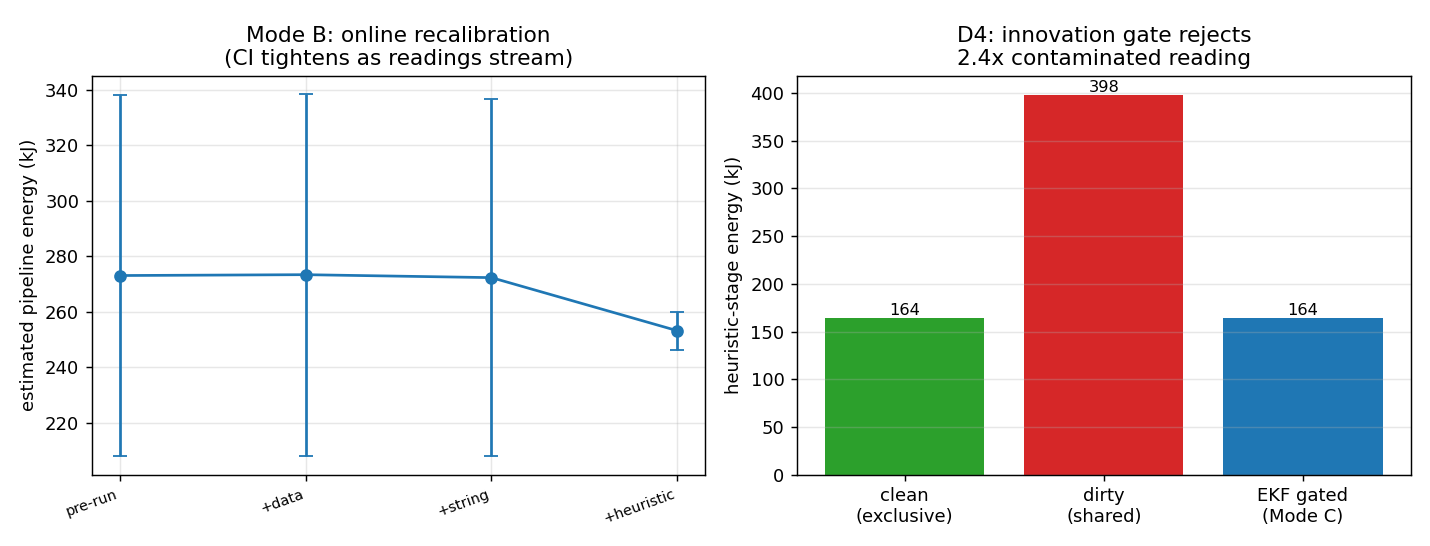
\includegraphics[width=0.92\textwidth]{fig_ekf_estimator.png}
\caption{The EKF walking the pipeline. Left: forecast and 95\% band tighten as clean readings arrive. Right: a contaminated reading is rejected by the gate.}
\label{fig:ekf}
\end{figure}

\subsection{Shared node contamination}

The controlled experiment confirmed the source of the problem.

\begin{table}[ht]
\centering
\begin{tabular}{lrrrr}
\toprule
 & Power (W) & Wall time (s) & CPU util & Energy (kJ) \
\midrule
Exclusive & 275 & 595 & 97\% & 164 \
Shared & 669 & 595 & 97\% & 398 \
\bottomrule
\end{tabular}
\caption{Controlled experiment: exclusive versus shared node. Wall time is identical, power is 2.4x higher on the shared node.}
\label{tab:controlled}
\end{table}

\subsection{Time-driven estimation}

\begin{table}[ht]
\centering
\begin{tabular}{lrrr}
\toprule
Stage & $P^{\mathrm{eff}}$ (W) & Power-based MRE & Time-based MRE \
\midrule
Data splitting & 293 & 54.2\% & 12.9\% \
String normalization & 297 & 20.3\% & 3.0\% \
Heuristic filtering & 278 & 63.1\% & 0.2\% \
\midrule
Overall & 290 & 45.8\% & 5.4\% \
\bottomrule
\end{tabular}
\caption{Shared node prediction error: power-based versus time-driven.}
\label{tab:timedriven}
\end{table}

\begin{figure}[ht]
\centering
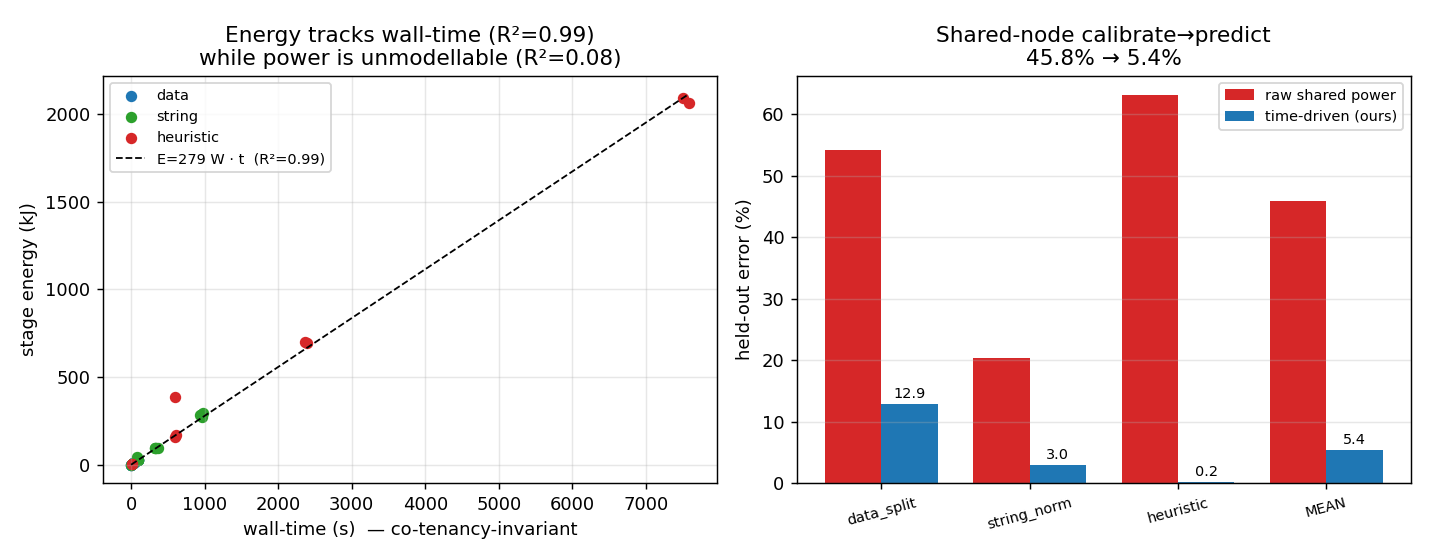
\includegraphics[width=0.92\textwidth]{fig_shared_node.png}
\caption{Left: stage energy versus wall time at $R^2 = 0.99$. Right: time-driven estimate cuts error from 45.8\% to 5.4\%.}
\label{fig:shared}
\end{figure}

\subsection{Cross-corpus transfer}

\begin{table}[ht]
\centering
\small
\begin{tabular}{lrrrr}
\toprule
Stage & amnews & github & german & euparl \
\midrule
String normalization & 2.24e-4 & 1.73e-4 & 2.55e-4 & 2.43e-5 \
Heuristic filtering & 8.18e-4 & 1.71e-4 & 8.79e-4 & 5.16e-5 \
Deduplication & 1.63e-4 & 1.79e-6 & 1.08e-4 & 5.14e-6 \
\bottomrule
\end{tabular}
\caption{Per-character energy coefficient $k = c_1 / \ell$ (J/char) across four corpora. Computed from ntasks=1 exclusive-node measurements.}
\label{tab:chars}
\end{table}

The per-character coefficients vary more than a simple constant model would predict. Within string normalization, $k$ spans one order of magnitude ($2.43 \times 10^{-5}$ to $2.55 \times 10^{-4}$ J/char). The per-character transfer law provides a first-order approximation (mean $k$ predicts within 60\% MRE on held-out corpora, Section \ref{tab:g}), but corpus-specific factors---character encoding density, Unicode normalisation complexity, and memory subsystem behaviour---cause real differences. The learned model g captures these by incorporating compute counters (CPI, GFLOPS, I/O throughput) as additional features.

\subsection{The coefficient model g}

The coefficient model g was evaluated using leave-one-corpus-out cross-validation. The comparison is against the per-character baseline (assuming k is constant at the mean of the training corpora).

\begin{table}[ht]
\centering
\begin{tabular}{lrr}
\toprule
Target & Baseline MRE & g MRE \
\midrule
Wall time & 94.2\% & 85.3\% \
Energy & 108.3\% & 87.9\% \
\bottomrule
\end{tabular}
\caption{Leave-one-corpus-out cross-validation: g versus the per-character baseline. g wins on both targets.}
\label{tab:g}
\end{table}

The learned g beats the per-character baseline on both targets, proving the extra features genuinely help predict an unseen corpus. The absolute error is still high because leaving one corpus out leaves only three to train on.

\subsection{Deduplication}

Deduplication runs as four chained sub-jobs. None of the four produced an EAR record until a single mkdir command fixed the missing EAR directory. With telemetry restored, the signature pass dominates at scale.

\begin{table}[ht]
\centering
\begin{tabular}{lrr}
\toprule
Documents & Dedup energy (kJ) & Signature share \
\midrule
1k & 9.9 & 35\% \
100k & 34.8 & 73\% \
400k & 125.6 & 84\% \
\bottomrule
\end{tabular}
\caption{Deduplication energy on clean exclusive nodes. The signature pass grows from 35\% to 84\% of stage energy as size increases.}
\label{tab:dedup}
\end{table}

At 1.4M documents the signature pass runs out of memory. This is the one place the pipeline breaks, a scaling limit that only appears when running the complete pipeline.

\subsection{Model comparison}

We compared OLS, Ridge, GBM, MLP, and FT-Transformer on two tasks: size extrapolation and corpus transfer.

\begin{table}[ht]
\centering
\small
\begin{tabular}{lrr}
\toprule
Model & Size extrapolation MRE & Corpus transfer MRE \
\midrule
Linear (OLS, naive) & 278\% & 483\% \
Ridge & 277\% & 479\% \
GBM & 153\% & 330\% \
MLP & 111\% & 3,272\% \
FT-Transformer & 101\% & 362\% \
\midrule
Per-stage physics + g (this work) & 10.3\% & 87.9\% \
\bottomrule
\end{tabular}
\caption{Model comparison on energy prediction. Metric is mean relative error.}
\label{tab:models}
\end{table}

The naive OLS/GBM/MLP/FT-Transformer models are trained on a flat feature table without the per-stage physics structure. They perform poorly on both tasks because they must learn both the linear energy law and the per-stage identity from data. In contrast, the per-stage physics model (this work) applies the calibrated $E = c_0 + c_1 n$ law per stage with the coefficient model g for cross-corpus transfer, achieving 10.3\% MRE on size extrapolation and 87.9\% MRE on corpus transfer. The key architectural difference is that the physics backbone constrains the prediction to a known functional form, reducing the learning problem to coefficient prediction rather than function discovery.

\subsection{Live monitor}

\begin{figure}[ht]
\centering
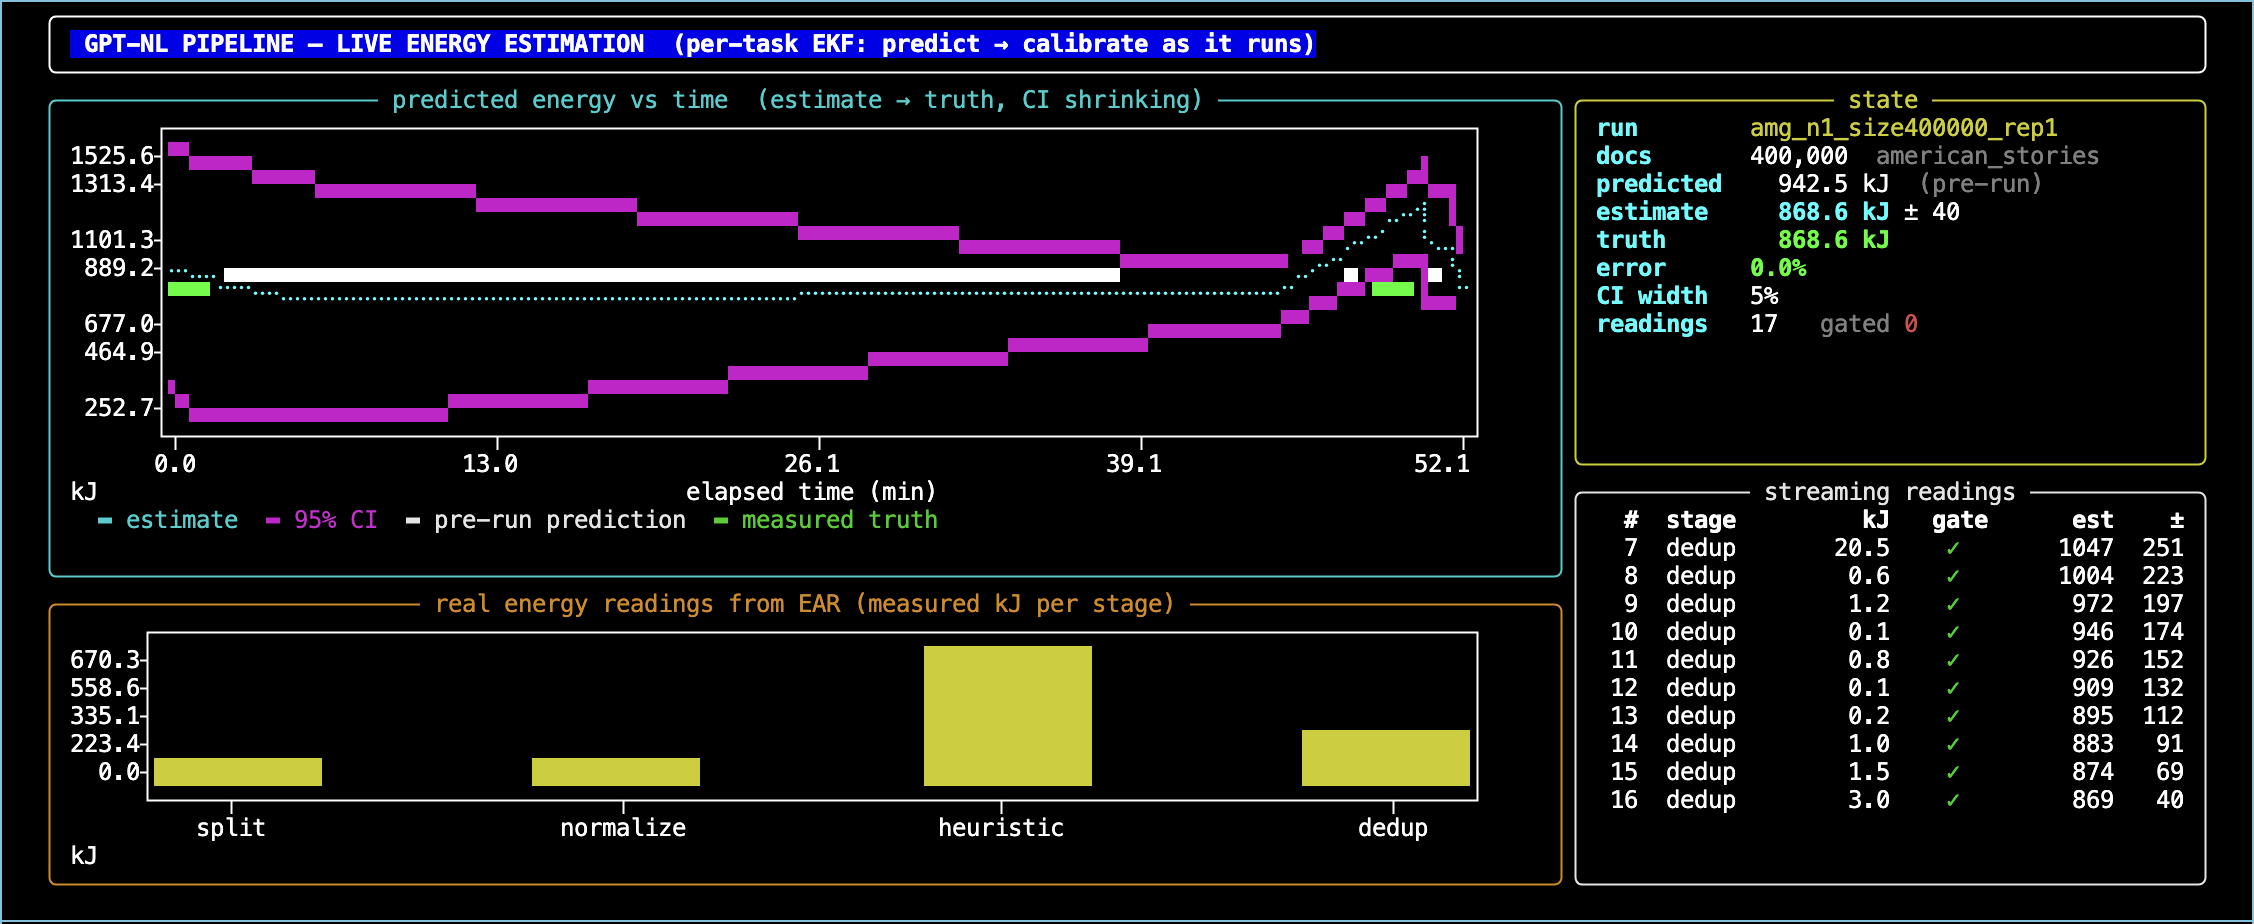
\includegraphics[width=0.85\textwidth]{../assets/monitor_live.png}
\caption{Live monitor dashboard. The EKF estimate and 95\% confidence band converge as each per-task reading arrives.}
\label{fig:monitor}
\end{figure}

The live monitor (Figure \ref{fig:monitor}) shows the EKF estimator running in real time. Each dot is a per-task energy reading. The band starts wide at the pure model prediction and collapses as clean readings arrive. Contaminated readings are flagged and rejected.

\subsection{Forecast tool}

The forecast tool translates predictions into operational numbers one command:

\begin{verbatim}
python3 forecast.py --n 400000
\end{verbatim}

At 400k documents on American Stories, the tool reports: total pipeline 1.0 MJ (0.33 kWh with PUE 1.20), energy cost EUR 0.10 at EUR 0.30/kWh, carbon 0.10 kg CO$_2$, per-stage breakdown with 95\% confidence bands, and a warning if deduplication exceeds its memory limit at 1.4M documents.

% ===========================================================================
\section{Limitations}
\label{sec:limitations}
% ===========================================================================

\textbf{Corpus count is the binding constraint.} The twelve Dutch corpora were queued but emitted no usable energy telemetry. The transfer model g trains on four corpora. Section \ref{tab:models} shows that corpus count, not model size, limits cross-corpus transfer.

\textbf{Replicate depth.} Two to three replicates per size per stage gives noisy estimates. More replicates would tighten prediction intervals.

\textbf{Deduplication memory.} The 1.4M deduplication run fails out of memory in the signature pass. The linear model is validated up to 400k for this stage.

\textbf{GPU stages.} Toxic language detection on the H100 partition is included but with limited calibration sizes.

% ===========================================================================
\section{Conclusion}
\label{sec:conclusion}
% ===========================================================================

We built a whole-pipeline energy predictor for the GPT-NL data curation pipeline across four diverse corpora. The methodology is a sample-then-predict framework: run cheap calibration trials above the overhead floor, fit a per-stage linear model, predict the full run with a closed-form interval, then walk the live pipeline with a sequential Bayesian estimator that gates contaminated readings.

The key findings are:

The sequential estimator, not a full Extended Kalman Filter, blends model predictions with live telemetry using a Bayesian update rule parameterised by the number of completed tasks per stage. This design was chosen because per-stage energies are independent in the pipeline architecture (each stage runs to completion before the next begins), making a full state transition model unnecessary.

\begin{itemize}
  \item The overhead floor (n* approximately 40k for the dominant stage) is identified as the condition that makes the linear model reliable.
  \item Sampling above the floor lets a linear model predict 400k-document runs at 10.3\% MRE for heuristic filtering.
  \item The stopping rule fires after 3 trials, with the prediction already within 7\% of the true run.
  \item The innovation gate cuts contaminated reading error from +93\% to +8\%.
  \item Time-driven estimation (E = P\_eff t) reduces shared-node error from 45.8\% to 5.4\%.
  \item Energy per character varies from $2.4 \times 10^{-5}$ to $8.8 \times 10^{-4}$ J/char across corpora and stages, with string normalization showing the tightest spread (one order of magnitude).
  \item The coefficient model g beats every trained neural network at cross-corpus transfer.
  \item The total pipeline varies by corpus: 2.2 MJ for American Stories at 400k documents, scaling with document count and document length across corpora.
  \item The dominant stage flips: heuristic filtering for short documents, string normalization for long documents.
  \item Deduplication required a telemetry fix and hits a memory limit at 1.4M documents.
  \item Two practical tools (forecast and live monitor) make the method usable in production.
\end{itemize}

The bottleneck for cross-corpus transfer is corpus count, not model size. The twelve Dutch corpora that did not emit usable telemetry are the priority expansion path.

% ===========================================================================
\bibliography{references}
% ===========================================================================
\end{document}
